% Condensed single-column build of the manuscript for a short-format venue. Compile
% with pdflatex + bibtex against refs.bib. This is the compressed companion of
% paper/manuscript.tex (the full preprint); both draw on the same refs.bib and figures.
\documentclass[11pt]{article}
\usepackage[utf8]{inputenc}
\usepackage[T1]{fontenc}
\usepackage{lmodern}
\usepackage[margin=1in]{geometry}
\usepackage{setspace}
\setstretch{1.5}
\usepackage{graphicx}
\usepackage{booktabs}
\usepackage{amsmath}
\usepackage{microtype}
\usepackage[hidelinks]{hyperref}
\usepackage[numbers,sort&compress]{natbib}
\usepackage{titlesec}
\titlespacing*{\section}{0pt}{6pt}{2pt}
\titlespacing*{\paragraph}{0pt}{4pt}{6pt}
\graphicspath{{../figures/}}
\pagestyle{plain}

\title{\vspace{-2.5em}Site-controlled evaluation reveals genuine killer-whale ecotype and
call-type structure in frozen audio-model embeddings}
% Correspondence email intentionally omitted from the public source; add on submission.
\author{Danielle Lesin \\ \small Georgia Institute of Technology, College of Computing}
\date{\vspace{-1em}}

\begin{document}
\maketitle
\vspace{-1.5em}

\begin{abstract}
\noindent Foundation-model embeddings are increasingly used to decode animal
vocalisations, but passive-acoustic archives confound the biological label with the
recording site. Encoding 27{,}934 public DCLDE~2026 killer-whale (\emph{Orcinus orca})
calls with a frozen AVES2 model \citep{palmer2025dclde,hagiwara2023aves}, we show pooled
ecotype decoding (balanced accuracy $0.910$) collapses to chance ($0.231$) under
leave-one-provider-out evaluation, while provider itself decodes at $0.948$; yet with site
held constant, ecotype stays strongly decodable ($0.889$--$0.973$). Catalogue-validated
call types are recoverable within site ($0.709$ for 14 SRKW types, $0.968$ for 18 NRKW
types) and, unlike ecotype, transfer across independent sites ($0.636$; $0.830$ on
unambiguous types). Call streams carry non-random first-order sequential structure over
tokens and over validated call types. On an independent animal-borne DTAG archive,
communicative calls predict the caller's movement-defined behavioural context with the
individual held out, across more than one context (foraging/non-foraging $0.770$;
foraging/travelling/resting $0.577$, chance $0.333$), with call-type$\times$context
selectivity and rate/loudness/echolocation controls \citep{holt2024masking_data}. On the
perception side, a re-analysis of a published conspecific playback experiment shows wild
killer whales respond selectively to broadcast calls---vocal reply to same-pod and not
different-pod playbacks ($6/6$ vs $0/6$, Fisher $p=0.002$), naive animals---and frozen AVES2
recovers the dialect call types that drive it (purity $0.439$ vs a $0.05$ null)
\citep{filatova2011playback,russianorca_catalogue}. The work is fully non-invasive and makes
no claim of meaning; its single response result re-analyses prior published playbacks and
tracks dialect membership, not call content.
\end{abstract}

\vspace{-0.5em}
\section{Introduction}
Killer whales produce stereotyped, group-distinctive pulsed calls whose repertoires vary
by ecotype and matriline \citep{ford1989,foote2008,filatova2015,yurk2002}. Self-supervised
audio models \citep{hagiwara2023aves,chen2022beats,robinson2024naturelm} make it tempting
to treat a frozen embedding plus a linear probe as evidence that a model ``understands'' a
species' calls. In passive-acoustic monitoring this is hazardous: the label (here ecotype)
is often collinear with the recording device and site, so a probe can score highly by
recognising the hydrophone, a shortcut well documented in bioacoustic deep learning
\citep{stowell2022,ghani2023}. We ask a narrow, auditable question---how much of the
apparent decodability is biological and how much is recording site---and answer it with
public data, frozen weights, explicit nulls, and a hash-frozen artifact, in the
conservative-claims spirit appropriate to interspecies-communication research
\citep{kershenbaum2024whyanimalstalk}. We make no claim of meaning or two-way
communication; the work that established context-specific dolphin signals required decades
of field data and in-situ playbacks \citep{sayigh2025nsw}. Our contribution is
methodological, not a new architecture: a confound-controlled evaluation protocol
(leave-one-provider-out site isolation, within-site discrimination, cross-site transfer), a
causal-attribution and negative-control battery, and an embedding analysis linking the
dialect space to a published playback response, all built around one frozen encoder so
every result is attributable to the representation under a single auditable protocol.

\vspace{-0.3em}
\section{Data and methods}
DCLDE~2026 is a public corpus distributed via NOAA/NCEI and a GCS mirror
\citep{palmer2025dclde,palmer2025dclde_data}; we use 27{,}934 call-level segments across
eight providers and four ecotypes (SRKW, an aggregated resident group, Bigg's, offshore),
each encoded once with frozen AVES2 (768-d, mean-pooled) and stored with provider, ecotype,
and time bounds. Raw audio is excluded from version control; the analysis consumes a
schema-validated, hash-frozen embedding artifact. \textbf{Ecotype probes (H1)} use pooled
5-fold CV (the site-confounded upper bound), leave-one-provider-out CV, and a label-shuffle
null. \textbf{Confound isolation (H4)} decodes provider directly, classifies ecotype
\emph{within} each provider (site held constant), and measures cross-site transfer.
\textbf{Call types} are Ford/Filatova catalogue codes recovered from the per-provider
annotations \citep{ford1989,filatova2015}; the full catalogue (8{,}552 detections) is
encoded and run within-provider and train-on-one/test-on-another. \textbf{Sequence
structure (H3)} quantises embeddings into a balanced 40-token vocabulary and tests
adjacent-call mutual information against a within-encounter order-shuffle null, with a
bigram-vs-unigram held-out comparison and a complementary masked-LM order test
\citep{vaswani2017attention,sharma2024}; the same test is re-run over validated catalogue
call types (Rung 4). \textbf{Behavioural context (H5)} re-analyses open animal-borne DTAG
deployments \citep{holt2024masking_data,tennessen2019}: tag audio is losslessly decoded,
communicative calls are detected ($0.5$--$10$\,kHz, clicks/echolocation rejected), and each
dive is labelled \emph{from movement only} (depth, jerk, ODBA \citep{wilson2006}); context
is decoded from the AVES2 call embeddings under leave-individual-out CV against a
label-permutation null. \textbf{Attribution} dissects the within-site signal (permutation
importance, top-$k$ vs random-$k$ knock-out, PCA curve) with structure-matched-noise,
feature-shuffle, and label-permutation negative controls. All runs are deterministic.

\vspace{-0.3em}
\section{Results}
\begin{table}[h]
\centering\small
\setlength{\tabcolsep}{4pt}
\begin{tabular}{llc}
\toprule
Head & Evaluation & Balanced acc.\ (chance) \\
\midrule
H1 & Pooled 5-fold CV & $0.910$ \\
H1 & Leave-one-provider-out & $0.231$ ($0.250$) \\
H4 & Provider decoding & $0.948$ ($0.125$) \\
H4 & Within-site ecotype (4 providers) & $0.889$--$0.973$ \\
H4 & Cross-site ecotype transfer & $0.529$ ($0.500$) \\
Call type & Within-VFPA, 14 SRKW types & $0.709$ ($0.071$) \\
Call type & Within-DFO\_CRP, 18 NRKW types & $0.968$ ($0.056$) \\
Call type & Cross-site VFPA$\to$SMRU & $0.636$ ($0.200$) \\
H3 & Adjacent-call MI vs shuffle & $1.91$ vs $1.65$ bits \\
Rung 4 & Validated N-call MI vs shuffle & $2.85$ vs $1.71$ bits \\
H5 & Foraging/non-foraging (LIO) & $0.770$ ($0.500$) \\
H5 & Three-way context (LIO) & $0.577$ ($0.333$) \\
H6 & Playback reply same- vs different-pod & $6/6$ vs $0/6$ ($p{=}0.002$) \\
H6 & FEROP dialect-type purity vs null & $0.439$ vs $0.05$ \\
\bottomrule
\end{tabular}
\caption{Headline results. LIO = leave-individual-out. All effects have permutation
$p\le 5\times10^{-3}$.}
\label{tab:five}
\end{table}

\paragraph{Ecotype: biology survives only with site control.} Pooled decoding reaches
$0.910$ but collapses to $0.231$ leave-one-provider-out, and provider decodes at $0.948$:
the pooled number is largely hydrophone recognition. With site held constant, ecotype stays
strongly decodable across four providers ($0.889$--$0.973$, all $p=5\times10^{-3}$), but
cross-site transfer is near chance ($0.529$)---the biology is real yet local
(Fig.~\ref{fig:h4}).

\paragraph{Call types are site-independent.} Frozen embeddings discriminate $14$ SRKW
S-call types within VFPA at $0.709$ and $18$ NRKW N-call types within DFO\_CRP at $0.968$
(both $p\approx0.005$), and a VFPA-trained classifier scores $0.636$ on the independent
SMRU site ($0.830$ on unambiguous types). Unlike ecotype, call-type identity transfers
across hydrophones---the control the ecotype boundary failed.

\paragraph{Sequence structure.} Adjacent-call mutual information is $1.91$ bits vs a
$1.65$-bit order-shuffle null ($p<10^{-3}$), $1.09$ bits after removing repetition; the same
holds over validated catalogue call types (NRKW $2.85$ vs $1.71$ bits). A prerequisite for
combinatorial coding, not evidence of meaning.

\paragraph{Communicative calls track behaviour, individual held out.} Across 22 tagged
whales ($10{,}834$ calls), calls predict movement-defined foraging context at $0.770$
(null $0.499$, $p=5\times10^{-3}$); a three-way foraging/travelling/resting decode reaches
$0.577$ (chance $0.333$) across the 20 whales visiting all three (Fig.~\ref{fig:ctx}).
Specific call types occur in specific contexts (Cram\'er's $V=0.40$ vs a within-individual
null of $0.08$, $p<10^{-3}$). Controls exclude trivial explanations: call rate alone decodes
at $0.536$, loudness at $0.577$, and dropping click-like clips leaves $0.749$.

\paragraph{Receivers respond to broadcast conspecific calls (perception side).} Re-analysing
a published conspecific playback experiment \citep{filatova2011playback}, wild killer whales
replied vocally to every same-pod playback and to none of the different-pod playbacks ($8/8$
vs $0/6$; $6/6$ vs $0/6$ after a pseudoreplication control, Fisher exact $p=0.002$), naive
free-ranging animals, often matching the played type \citep{miller2004repertoires}. Encoding
the public FEROP catalogue \citep{russianorca_catalogue} with frozen AVES2, leave-one-out
1-NN call-type purity is $0.439$ across 19 dialect types vs a $0.050$ label-shuffle null
($p=10^{-3}$): the encoder represents the dialect space that drives the response. The
behavioural experiment is prior work; the response tracks dialect membership, not call content.
The criterion is corroborated across independent broadcast-response datasets
\citep{selbmann2026aversive,bowers2018,miller2004repertoires}. On the production side, the
recovered catalogue call types specialise across foraging vs socialising---$72\%$ ($13/18$
NRKW/SRKW types) are single-context specialists (foraging: N4, N9; socialising: the multi-pod
two-voiced/identity calls), context labels from published ethograms, not embeddings
\citep{ford1989,foote2008}.

\paragraph{The signal is distributed and not an artifact.} On the within-site SRKW/TKW
decode ($0.979$), no small dimension set is necessary (top-$k$ knock-out stays $0.93$--$0.97$
through $k{=}200$; one dimension is at chance; $\sim\!100$ PCA components reach $0.91$), and
matched-noise ($0.536$), feature-shuffle ($0.505$), and label-permutation ($0.503$,
$p=8\times10^{-3}$) controls all sit near chance: genuine joint structure, not a gamed leak.

\begin{figure}[h]
\centering
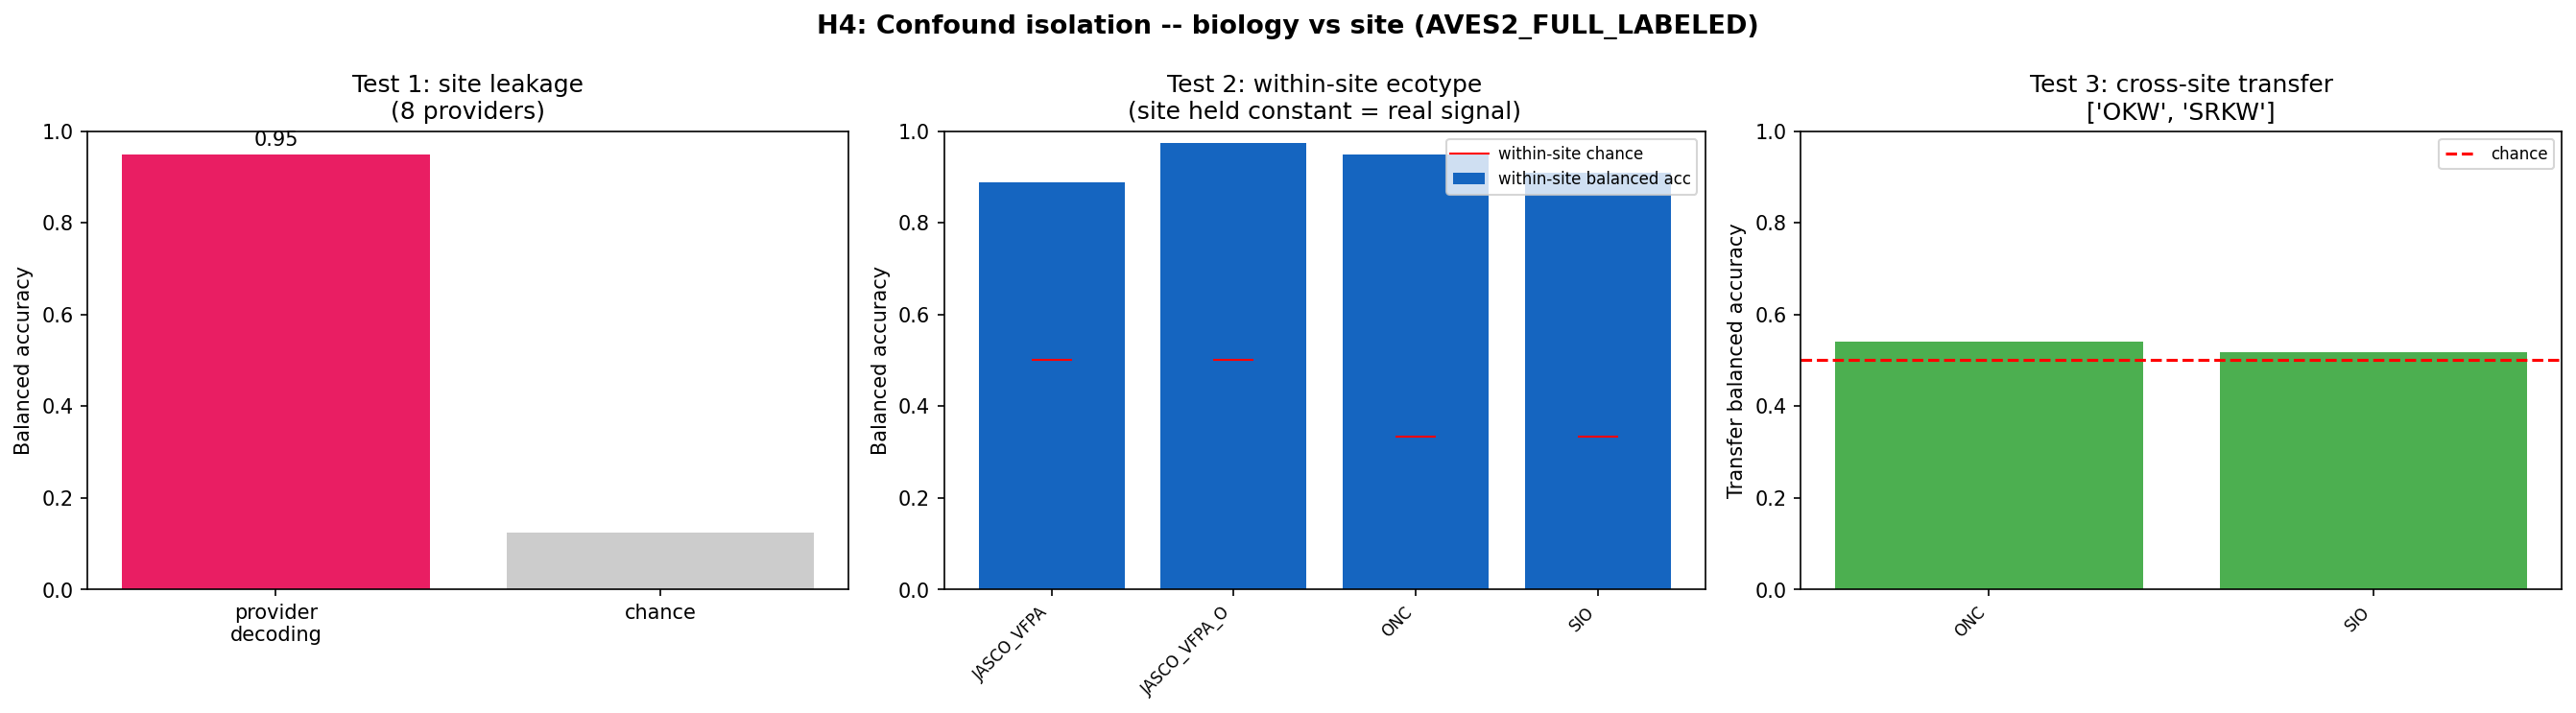
\includegraphics[width=0.9\linewidth]{h4_confound_aves2_full_labeled.png}
\caption{Provider decodes at $0.948$ (left); ecotype is strongly decodable within each fixed
site (middle); cross-site transfer is near chance (right). The signal is real but local.}
\label{fig:h4}
\end{figure}

\begin{figure}[h]
\centering
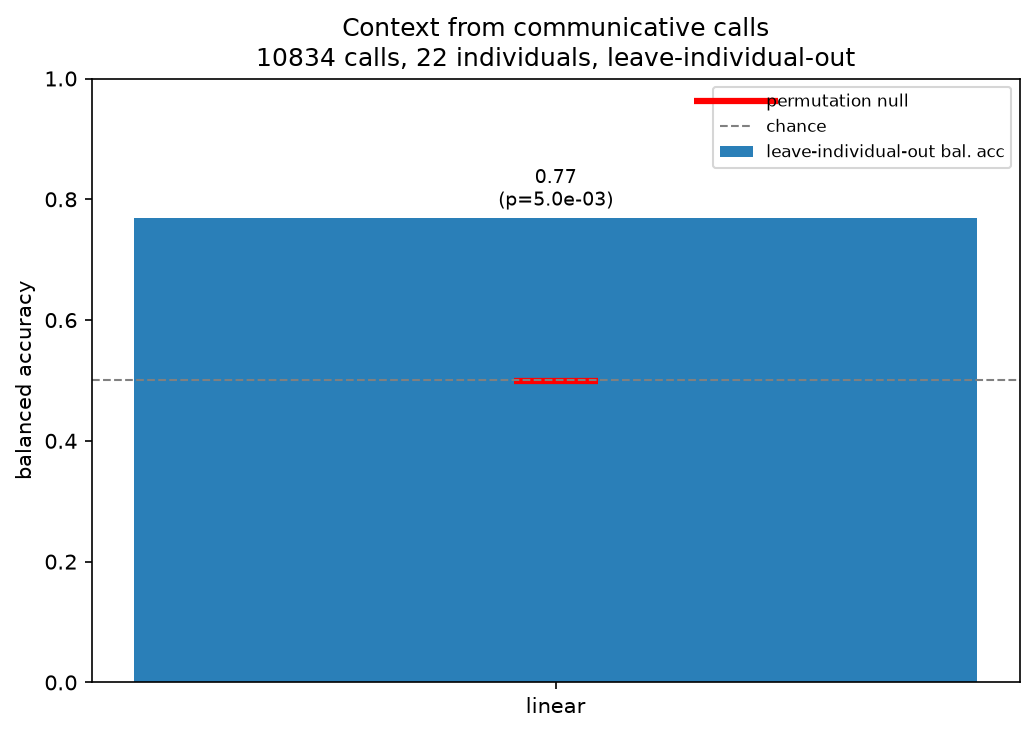
\includegraphics[width=0.78\linewidth]{context_decode.png}
\caption{DTAG H5: communicative calls predict movement-defined foraging context at $0.770$
under leave-individual-out CV (null $0.499$). The label uses depth/acceleration only, so it
is independent of the decoded audio.}
\label{fig:ctx}
\end{figure}

\vspace{-0.3em}
\section{Limitations and confidence}
Pooled accuracy is a site-confounded upper bound, not reported as biology. Call-type labels
are detection-level and correlate with pod/matriline, so this is call-type discrimination,
not meaning; the SMRU transfer set is small. The H5 context labels are movement-only
proxies and the on-tag call-type clusters are soft; a behavioural-context decode could
reflect arousal rather than content, though the call-type$\times$context selectivity and the
loudness control ($0.577$) argue against a pure-arousal account. Non-acoustic channels
(posture, surface behaviour, touch) are not captured, which bounds interpretation but cannot
inflate an acoustic decode or a response to an acoustic broadcast. \emph{Calibrated
confidence}---\textbf{high}: site-controlled ecotype/call-type structure and cross-site
call-type transfer; \textbf{medium--high}: context-specific production across more than one
movement-defined context, individual held out; \textbf{medium--high}: a dialect-selective receiver
response to broadcast conspecific calls (H6), by re-analysis of a prior published playback
(clean differential response, corroborated across independent datasets, but small conspecific $n$); \textbf{no claim}: referential meaning, or that
the receiver response is governed by call content rather than dialect membership---which
requires a controlled content-isolating playback \citep{deecke2005,sayigh2025nsw}.

\vspace{-0.3em}
\section{Reproducibility}
All code, a hash-frozen artifact, per-head metrics JSON, and figures are released with exact
commands; every reported number regenerates from the frozen artifact. Raw audio and tag
archives are downloaded from public sources and excluded from version control.

{\small
\bibliographystyle{plainnat}
\bibliography{refs}
}
\end{document}
